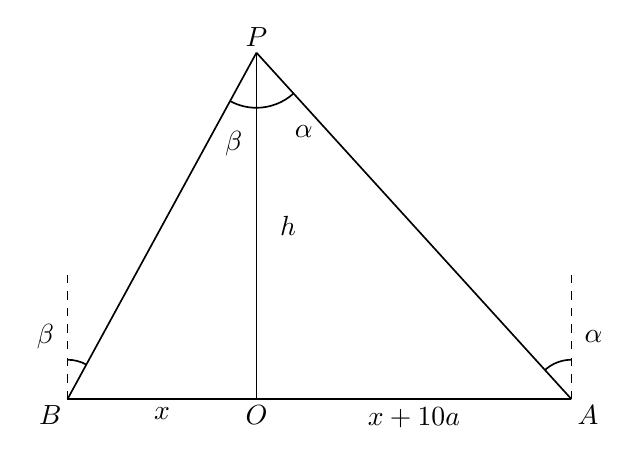
\begin{tikzpicture}[x=2cm,y=2cm,font=\normalsize,
 geometry edge/.style={solid,line width=.6pt},
 geometry mark/.style={solid,line width=.6pt},
 geometry label/.style={font=\normalsize,inner sep=0pt}]
\coordinate (P) at (0,2.2);
\coordinate (O) at (0,0);
\coordinate (B) at (-1.2,0);
\coordinate (A) at (2,0);
\coordinate (BN) at (-1.2,0.8);
\coordinate (AN) at (2,0.8);
\draw[geometry edge] (P)--(B);
\draw[geometry edge] (P)--(A);
\draw[geometry edge] (B)--(O);
\draw[geometry edge] (O)--(A);
\draw[geometry edge] (P)--(O);
\draw[geometry edge,dashed] (B)--(BN);
\draw[geometry edge,dashed] (A)--(AN);
\draw[geometry mark] (P) ++(241.389540334035:7mm) arc[start angle=241.389540334035,end angle=270.000000000000,radius=7mm];
\draw[geometry mark] (P) ++(270.000000000000:7mm) arc[start angle=270.000000000000,end angle=312.273689006094,radius=7mm];
\draw[geometry mark] (B) ++(61.389540334035:5mm) arc[start angle=61.389540334035,end angle=90.000000000000,radius=5mm];
\draw[geometry mark] (A) ++(90.000000000000:5mm) arc[start angle=90.000000000000,end angle=132.273689006094,radius=5mm];
\node[font=\normalsize] at (-0.145,1.62) {$\beta$};
\node[font=\normalsize] at (0.30,1.70) {$\alpha$};
\node[font=\normalsize] at (-1.34,0.4) {$\beta$};
\node[font=\normalsize] at (2.14,0.4) {$\alpha$};
\node[font=\normalsize] at (0.2,1.1) {$h$};
\node[font=\normalsize,below=3pt,inner sep=0pt] at (-0.6,0) {$x$};
\node[font=\normalsize,below=3pt,inner sep=0pt] at (1,0) {$x+10a$};
\node[geometry label,above=2pt] at (P) {$P$};
\node[geometry label,below=2pt] at (O) {$O$};
\node[geometry label,below left=2pt] at (B) {$B$};
\node[geometry label,below right=2pt] at (A) {$A$};
\end{tikzpicture}
